\section{Revue de la littérature}

  \subsection{Revue des travaux de recherche existants } 
Avant de commencer notre projet, nous avons effectué une revue des travaux de recherche existants dans le domaine des L-systèmes. Nous avons consulté les ressources mises à disposition par notre professeur, ce qui s'est avéré très utile pour notre projet. Cette recherche nous a permis de découvrir la théorie des L-systèmes développée par Aristid Lindenmayer, un biologiste hongrois dans les années 60. Cette théorie permet de décrire la croissance des plantes et des organismes biologiques. Nous avons également découvert qu'il existe plusieurs types de L-systèmes qui diffèrent d'un système à un autre, principalement par la manière dont un système donné interprète les règles fournies par l'utilisateur.
        	\begin{figure}[h!]
  \centering
  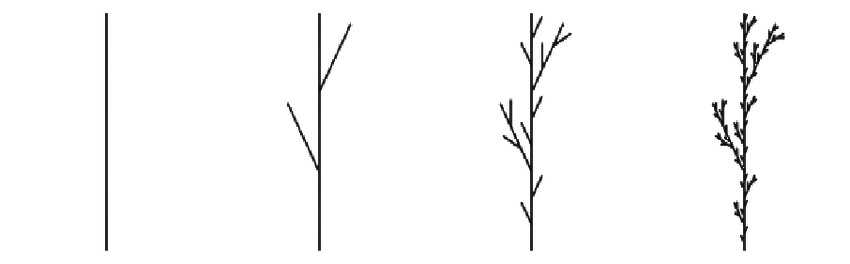
\includegraphics[width=0.5\textwidth]{images/plante.png}
  \caption{generation d'une plante avec un L-systeme}
  \label{fig:plante}
\end{figure}

       En approfondissant nos recherches, nous avons découvert qu'il existe plusieurs algorithmes pour la réécriture de chaînes et la génération de graphiques 2D et 3D à partir des L-systèmes. Nous avons également constaté que les L-systèmes sont largement utilisés dans divers domaines tels que les jeux vidéos, les films, la biologie, l'architecture et l'art. Nous avons également identifié les tendances actuelles dans la recherche sur les L-systèmes, notamment les L-systèmes paramétriques, les L-systèmes interactifs et les L-systèmes évolutifs. Ces types de L-systèmes sont plus complexes et visent à créer des structures plus grandes et plus détaillées.

	 \label{source}voici quelque exemple: 
\begin{itemize}
    \item \textbf{L-systèmes déterministes:}
    Les L-systèmes déterministes sont les plus simples et les plus courants. Ils utilisent un ensemble de règles de production fixes et déterministes pour remplacer les symboles de l'axiome initial. La croissance de la structure est entièrement déterminée par les règles de production et l'état initial.

    \textbf{Exemple : Le flocon de von Koch}\\
    \begin{center}
          \fbox{
       
        \begin{minipage}{0.4\textwidth}
        \centering
          Axiome : F--F--F\\
        Règles : F -> F+F--F+F\\
        Angle : 60 degrés
        \end{minipage}
    }
    \end{center}
    
    \item \textbf{L-systèmes stochastiques:}\\
    Les L-systèmes stochastiques introduisent une composante aléatoire dans les règles de production. Chaque symbole peut avoir plusieurs règles de production, chacune avec une certaine probabilité d'être choisie. Cela permet de générer des structures plus variées et plus naturelles.

    \textbf{Exemple : Plante stochastique}\\
    
   
    \begin{center}
          \fbox{
       
        \begin{minipage}{0.8\textwidth}
        \centering
           Axiome : X\\
            Règles : X -> F-[[X]+X]+F[+FX]-X avec probabilité 0.5\\
            X -> F+[[X]-X]-F[-FX]+X avec probabilité 0.5\\
            F -> FF\\
            Angle : 25 degrés
        \end{minipage}
    }
    \end{center}
    \item \textbf{L-systèmes contextuels:}\\
    Les L-systèmes contextuels tiennent compte du contexte des symboles pour déterminer les règles de production à appliquer. Les règles de production ont des préconditions qui doivent être remplies pour qu'elles puissent être appliquées. Cela permet de créer des structures plus complexes et plus réalistes.

    \textbf{Exemple : L-système contextuel simple\\}
    
    \begin{center}
          \fbox{
       
        \begin{minipage}{0.5\textwidth}
        \centering
           Axiome : A[B]C\\
        Règles : B -> X dans le contexte A \_ C (B est remplacé par X si B est entre A et C)\\
        Angle : Non applicable
        \end{minipage}
    }
    \end{center}
\end{itemize}



  
  
   
 \subsection{Présentation des concepts clés des L-systèmes}   

    \begin{itemize}
        \item Alphabet : Un L-système utilise un ensemble fini de symboles, appelé alphabet, pour représenter les éléments de base de la structure à modéliser ,les alphabets sont représenter dans notre projet  sous forme d'un set ou une liste de "{A,......,Z}" dans la classe "Alphabet.java".
        \item Axiome : L'axiome est la chaîne initiale à partir de laquelle le L-système commence son processus de réécriture. Il représente généralement l'état initial de la structure à modéliser , représenter par un string dans notre projet.
        \item Règles de production : Les règles de production définissent comment les symboles de l'axiome ou des chaînes dérivées sont remplacés par d'autres symboles ou séquences de symboles. Ces règles déterminent la manière dont la structure évolue au fil des réécritures successives , ce qu'on appelle le parser représenter par un dictionnaire (cle,valeur) "HashMap" dans la classe "Rule.java".[\ref{hash}]
        \item Processus de réécriture : Le processus de réécriture consiste à appliquer les règles de production à la chaîne actuelle de manière répétée, en remplaçant chaque symbole par la séquence de symboles correspondante définie par les règles de production. Chaque application des règles de production est appelée une "itération" ou "génération".
    \end{itemize}

    

    

    

